\documentclass[11pt,a4paper]{article}
\usepackage[margin=2.4cm]{geometry}
\usepackage{amsmath}
\usepackage{fontspec}
\usepackage{microtype}
\usepackage{booktabs}
\usepackage{graphicx}
\usepackage{enumitem}
\usepackage{titlesec}
\usepackage[hidelinks]{hyperref}
\usepackage{fancyhdr}

\setmainfont{TeX Gyre Termes}
\setmonofont{TeX Gyre Cursor}[Scale=0.86]

\titleformat{\section}{\large\bfseries}{S\thesection}{0.7em}{}
\titlespacing*{\section}{0pt}{2.2ex}{1ex}
\pagestyle{fancy}\fancyhf{}
\fancyhead[L]{\small Supplementary material}
\fancyhead[R]{\small Deploying LLM Inference on a Repurposed UMA APU}
\fancyfoot[C]{\small\thepage}
\renewcommand{\headrulewidth}{0.4pt}

\setlength{\parskip}{0.6ex}
\setlength{\parindent}{0pt}

\begin{document}

\begin{center}
{\Large\bfseries Supplementary Material}\\[0.6ex]
{\large Deploying LLM Inference on a Repurposed UMA APU:\\
Transferable Lessons from a Vulkan-Only, 16\,GB Edge Platform}\\[1.2ex]
{Artur Andrzejczak}\\[0.8ex]
\end{center}

\noindent This document holds the per-run and per-cell detail referred to from the
main text.  Every number here comes from the released measurement data
in the project repository; the file backing each table is named in its
caption.  Raw logs, harnesses and the full JSON results are in the same
repository.  Unless stated otherwise, all measurements are from the
verified-stock 24-CU configuration under Ollama~0.20.0 /
llama.cpp~b9265 at the 16\,GiB pool
(\texttt{ttm.pages\_limit}=4\,194\,304).

\tableofcontents

%=====================================================================
\section{Heap Placement Under \texttt{GGML\_VK\_PREFER\_HOST\_MEMORY}}
%=====================================================================

On a unified-memory device the Vulkan allocator can place model weights
in either the device-local heap or the host-visible heap.  Setting
\texttt{GGML\_VK\_PREFER\_HOST\_MEMORY=1} forces the latter.
Table~\ref{tab:s-heap} gives the A/B on two models, two llama.cpp builds
and three prefill lengths, one run per cell.

\begin{table}[h]
\centering\small
\caption{Wall-clock time by heap placement (seconds; one
\texttt{llama-bench} invocation per cell with two internal repeats;
lower is better).  Source: \texttt{results-prefer-host-mem.json}.}
\label{tab:s-heap}
\begin{tabular}{@{}llrrrr@{}}
\toprule
\textbf{Build} & \textbf{Model} & \textbf{Prefill} & \textbf{Default} & \textbf{Prefer host} & \textbf{Change} \\
\midrule
b8200 & \texttt{deepseek-r1-14b}    &  2048 &  78.66 &  69.55 & $-11.6\,\%$ \\
b8200 & \texttt{deepseek-r1-14b}    &  4096 & 127.50 & 119.68 & $-6.1\,\%$ \\
b8200 & \texttt{deepseek-r1-14b}    & 16384 & 631.77 & 637.45 & $+0.9\,\%$ \\
b8200 & \texttt{moe-coder-30b-iq2m} &  2048 &  56.89 &  49.52 & $-13.0\,\%$ \\
b8200 & \texttt{moe-coder-30b-iq2m} &  4096 &  79.43 &  74.14 & $-6.7\,\%$ \\
b8200 & \texttt{moe-coder-30b-iq2m} & 16384 & 358.62 & 356.56 & $-0.6\,\%$ \\
\midrule
b9165 & \texttt{deepseek-r1-14b}    &  2048 &  75.42 &  68.58 & $-9.1\,\%$ \\
b9165 & \texttt{deepseek-r1-14b}    &  4096 & 125.18 & 115.66 & $-7.6\,\%$ \\
b9165 & \texttt{deepseek-r1-14b}    & 16384 & 632.90 & 632.74 & $-0.0\,\%$ \\
b9165 & \texttt{moe-coder-30b-iq2m} &  2048 &  56.68 &  48.78 & $-13.9\,\%$ \\
b9165 & \texttt{moe-coder-30b-iq2m} &  4096 &  79.60 &  74.11 & $-6.9\,\%$ \\
b9165 & \texttt{moe-coder-30b-iq2m} & 16384 & 362.99 & 358.35 & $-1.3\,\%$ \\
\bottomrule
\end{tabular}
\end{table}

The effect depends on prefill length.  At 2048 and 4096 tokens host
placement is faster in all eight cells, by 6.1 to 13.9\,\%, and the
advantage shrinks as prefill grows.  At 16384 tokens it is gone: three
cells move by less than 1.5\,\% and one is slower with host placement.
Both builds behave the same way, so the pattern follows the prefill
length, not the llama.cpp version.  A single run per cell does
not separate a small effect from run-to-run scatter, which is why only
the 2048 and 4096 tiers, where the gap is several times the dispersion
seen elsewhere in this paper, support a direction.  The canonical
measurements leave the variable at its default.

%=====================================================================
\section{KV-Cache Footprint by Width}
%=====================================================================

KV-cache bytes per token follow from the model geometry: two tensors
(keys and values) per layer, $n_{\text{kv}}$ key/value heads of
dimension $d_{\text{head}} = n_{\text{embd}} / n_{\text{head}}$, at the
element width of the cache.  Table~\ref{tab:s-kvfoot} evaluates this for
the models whose metadata was read for the head-count analysis of the
main text.

\begin{table}[h]
\centering\small
\caption{KV-cache footprint at 24\,576 tokens of context, computed from
GGUF metadata.  Source: \texttt{step-a13-head-counts.json}, harness
\texttt{heads.py}.}
\label{tab:s-kvfoot}
\begin{tabular}{@{}lrrrrrr@{}}
\toprule
& & & & \multicolumn{3}{c}{\textbf{Footprint at 24K (GiB)}} \\
\cmidrule(l){5-7}
\textbf{Model} & \textbf{Layers} & \textbf{KV heads} & \textbf{$d_{\text{head}}$}
  & \textbf{FP16} & \textbf{Q8\_0} & \textbf{Q4\_0} \\
\midrule
\texttt{qwen2.5:0.5b}       & 24 & 2 &  64 & 0.28 & 0.14 & 0.07 \\
\texttt{qwen2.5:1.5b}       & 28 & 2 & 128 & 0.66 & 0.33 & 0.16 \\
\texttt{qwen2.5:3b}         & 36 & 2 & 128 & 0.84 & 0.42 & 0.21 \\
\texttt{qwen2.5:7b}         & 28 & 4 & 128 & 1.31 & 0.66 & 0.33 \\
\texttt{qwen2.5:14b}        & 48 & 8 & 128 & 4.50 & 2.25 & 1.12 \\
\texttt{qwen2.5-coder:1.5b} & 28 & 2 & 128 & 0.66 & 0.33 & 0.16 \\
\bottomrule
\end{tabular}
\end{table}

The columns use the nominal element widths of 16, 8 and 4 bits;
llama.cpp's Q8\_0 and Q4\_0 blocks add a 16-bit scale per 32 elements,
so the stored caches are 8.5 and 4.5 bits per element and the Q4\_0
footprint is 0.28 of FP16, not 0.25.  That factor is what buys the
longer context tiers on a fixed 16\,GiB pool.  The main
text reports the quality cost of that choice.

%=====================================================================
\section{Downstream Task Accuracy: HellaSwag and Winogrande}
%=====================================================================

The main text states that neither benchmark resolves the sub-2\,\%
perplexity effect on models that do not collapse.  Table~\ref{tab:s-tasks}
gives the per-cell accuracies behind that statement, and
Table~\ref{tab:s-mcnemar} the paired test on the HellaSwag outcomes.

\begin{table}[h]
\centering\small
\caption{Accuracy over 400 randomised tasks per cell at 2048 context,
flash attention on.  Source: \texttt{step-a7-p2-accuracy.json},
recovered from the raw logs in \texttt{a7-raw/}.}
\label{tab:s-tasks}
\begin{tabular}{@{}llrrr@{}}
\toprule
\textbf{Benchmark} & \textbf{Model} & \textbf{FP16 KV} & \textbf{Q4\_0 KV} & \textbf{Change} \\
\midrule
HellaSwag   & \texttt{phi4-mini}     & 70.00\,\% & 68.75\,\% & $-1.25$\,pp \\
HellaSwag   & \texttt{qwen3-14b}     & 78.25\,\% & 78.25\,\% & $0.00$\,pp \\
HellaSwag   & \texttt{qwen3-8b} (Q4\_K\_M) & 74.25\,\% & 75.00\,\% & $+0.75$\,pp \\
HellaSwag   & \texttt{qwen3-8b} (Q8\_0)    & 75.25\,\% & 74.75\,\% & $-0.50$\,pp \\
\midrule
Winogrande  & \texttt{phi4-mini}     & 72.50\,\% & 71.00\,\% & $-1.50$\,pp \\
Winogrande  & \texttt{qwen3-8b} (Q4\_K\_M) & 68.00\,\% & 68.75\,\% & $+0.75$\,pp \\
Winogrande  & \texttt{qwen3-8b} (Q8\_0)    & 66.50\,\% & 66.50\,\% & $0.00$\,pp \\
\bottomrule
\end{tabular}
\end{table}

\begin{table}[h]
\centering\small
\caption{Paired McNemar test on the HellaSwag per-task outcomes,
continuity-corrected.  Discordant pairs are tasks answered correctly
under one cache width and not the other.  Source:
\texttt{step-a7-p2-accuracy.json}.}
\label{tab:s-mcnemar}
\begin{tabular}{@{}lrrr@{}}
\toprule
\textbf{Model} & \textbf{FP16 only} & \textbf{Q4\_0 only} & $\boldsymbol{\chi^2}$ \\
\midrule
\texttt{phi4-mini}           & 10 &  5 & 1.07 \\
\texttt{qwen3-14b}           &  3 &  3 & 0.17 \\
\texttt{qwen3-8b} (Q4\_K\_M) &  6 &  9 & 0.27 \\
\texttt{qwen3-8b} (Q8\_0)    &  7 &  5 & 0.08 \\
\bottomrule
\end{tabular}
\end{table}

All four values fall well below the 3.84 threshold for significance at
$p=0.05$ with one degree of freedom.  Accuracy moves by at most
1.5~percentage points and the sign is not consistent, so 400 tasks do
not resolve an effect of this size.  This bounds the short-context
significance of the perplexity penalty; it does not contradict it.

The sweep harness did not parse the score line printed by
\texttt{llama-perplexity} and recorded these cells as failed in
\texttt{step-a7-broad.json}.  The runs themselves completed, and the
values above were read back from the retained logs.

%=====================================================================
\section{Multi-Hop Reasoning at the 1024-Token Budget}
%=====================================================================

The main text reports that raising the output budget from 300 to 1024
tokens splits an apparent tie between models.  Table~\ref{tab:s-multihop}
gives the per-task counts.

\begin{table}[h]
\centering\small
\caption{Multi-hop pass counts at a 1024-token output budget, three runs
per cell.  Source: \texttt{step-g6-multihop.json} and
\texttt{step-g6-multihop-extra.json}.}
\label{tab:s-multihop}
\begin{tabular}{@{}llrr@{}}
\toprule
\textbf{Model} & \textbf{Context} & \textbf{Budget chain} & \textbf{Population chain} \\
\midrule
\texttt{qwen3.5:9b}      & 16K & 3/3 & 3/3 \\
\texttt{qwen3.5:9b}      & 32K & 3/3 & 3/3 \\
\texttt{qwen3.5-35b-a3b} & 16K & 3/3 & 3/3 \\
\texttt{qwen3.5-35b-a3b} & 32K & 3/3 & 3/3 \\
\texttt{phi4-mini}       & 16K & 2/3 & 0/3 \\
\texttt{phi4-mini}       & 32K & 0/3 & 0/3 \\
\bottomrule
\end{tabular}
\end{table}

The two long-context-capable models answer every item at both depths.
\texttt{phi4-mini} passes neither task at 32K and only part of one at
16K, so the longer budget separates a capability limit from an output
truncation artefact.

%=====================================================================
\section{Multi-Needle Retrieval by Depth}
%=====================================================================

Five fixed-content codes were planted at even depths through the
prompt.  Table~\ref{tab:s-needle} gives the per-needle recall across two
runs per tier.

\begin{table}[h]
\centering\small
\caption{Per-needle recall, two runs per tier; each entry is the number
of runs in which that code was recovered.  Source:
\texttt{step-multi-needle.json}.}
\label{tab:s-needle}
\begin{tabular}{@{}lrrrrrr@{}}
\toprule
\textbf{Model} & \textbf{Context} & \textbf{N1} & \textbf{N2} & \textbf{N3} & \textbf{N4} & \textbf{N5} \\
\midrule
\texttt{qwen3.5:9b}        &  32K & 2 & 2 & 2 & 2 & 2 \\
\texttt{qwen3.5:9b}        &  64K & 2 & 2 & 2 & 2 & 2 \\
\texttt{qwen3.5:9b}        & 128K & 2 & 2 & 2 & 2 & 2 \\
\texttt{granite-4.0-h-tiny} &  32K & 2 & 2 & 2 & 2 & 2 \\
\texttt{granite-4.0-h-tiny} &  64K & 2 & 2 & 2 & 2 & 2 \\
\texttt{granite-4.0-h-tiny} & 128K & 2 & 2 & 2 & 2 & 2 \\
\texttt{deepseek-r1-14b}   &  32K & 2 & 2 & 2 & 2 & 2 \\
\texttt{deepseek-r1-14b}   &  64K & 2 & 2 & 2 & 2 & 2 \\
\texttt{gemma4-latest}     &  32K & 0 & 0 & 0 & 0 & 0 \\
\texttt{gemma4-latest}     &  64K & 0 & 0 & 0 & 0 & 0 \\
\texttt{gemma4-latest}     & 128K & 0 & 0 & 0 & 0 & 0 \\
\bottomrule
\end{tabular}
\end{table}

Recall does not decay with depth on the models that retrieve at all.
\texttt{qwen3.5:9b} and \texttt{granite-4.0-h-tiny} recover all five
codes at every tier through 128K, and \texttt{deepseek-r1-14b} does so
at both tiers it reaches.  \texttt{deepseek-r1-14b}
has no 128K row because that tier exceeds the working-set guard.  The
Gemma-4 community fork returns chain-of-thought instead of the requested
code at every depth, which the scorer counts as a miss.

%=====================================================================
\section{40-CU Speed-Up by Context Tier}
%=====================================================================

Table~\ref{tab:s-cutier} pairs the two compute-unit arms cell by cell on
the filled-context ladder.

\begin{table}[h]
\centering\small
\caption{Generation speed (tok/s, median of three runs) on the 24-CU and
40-CU arms with the per-cell ratio.  Same sources as Table~15 of the main
text: \texttt{results-phase-d-24cu-ladder/} and
\texttt{results-phase-d-stage2/}.}
\label{tab:s-cutier}
\begin{tabular}{@{}lrrrr@{}}
\toprule
\textbf{Model} & \textbf{Context} & \textbf{24 CU} & \textbf{40 CU} & $\boldsymbol{\Delta}$ \\
\midrule
\texttt{deepseek-r1-14b} & 4K & 18.6 & 27.4 & 1.48$\times$ \\
\texttt{deepseek-r1-14b} & 8K & 16.6 & 24.5 & 1.48$\times$ \\
\texttt{deepseek-r1-14b} & 16K & 13.5 & 20.2 & 1.49$\times$ \\
\texttt{deepseek-r1-14b} & 24K & 11.4 & 17.6 & 1.55$\times$ \\
\midrule
\texttt{qwen3.5:9b} & 4K & 23.1 & 31.3 & 1.35$\times$ \\
\texttt{qwen3.5:9b} & 8K & 22.5 & 30.5 & 1.36$\times$ \\
\texttt{qwen3.5:9b} & 16K & 21.4 & 29.2 & 1.36$\times$ \\
\texttt{qwen3.5:9b} & 24K & 19.4 & 26.4 & 1.36$\times$ \\
\texttt{qwen3.5:9b} & 32K & 18.6 & 25.6 & 1.38$\times$ \\
\texttt{qwen3.5:9b} & 48K & 17.7 & 25.1 & 1.41$\times$ \\
\texttt{qwen3.5:9b} & 64K & 16.3 & 23.4 & 1.43$\times$ \\
\midrule
\texttt{granite-4.0-h-tiny} & 4K & 102.6 & 126.0 & 1.23$\times$ \\
\texttt{granite-4.0-h-tiny} & 8K & 101.2 & 121.8 & 1.20$\times$ \\
\texttt{granite-4.0-h-tiny} & 16K & 98.9 & 122.6 & 1.24$\times$ \\
\texttt{granite-4.0-h-tiny} & 24K & 96.4 & 116.6 & 1.21$\times$ \\
\texttt{granite-4.0-h-tiny} & 32K & 94.3 & 115.4 & 1.22$\times$ \\
\texttt{granite-4.0-h-tiny} & 48K & 90.0 & 113.5 & 1.26$\times$ \\
\texttt{granite-4.0-h-tiny} & 64K & 86.4 & 110.0 & 1.27$\times$ \\
\midrule
\texttt{gemma4-latest} & 4K & 26.7 & 30.9 & 1.16$\times$ \\
\texttt{gemma4-latest} & 8K & 27.4 & 31.1 & 1.14$\times$ \\
\texttt{gemma4-latest} & 16K & 25.5 & 30.1 & 1.18$\times$ \\
\texttt{gemma4-latest} & 24K & 24.3 & 28.8 & 1.19$\times$ \\
\texttt{gemma4-latest} & 32K & 22.6 & 27.2 & 1.20$\times$ \\
\texttt{gemma4-latest} & 48K & 21.2 & 26.1 & 1.23$\times$ \\
\texttt{gemma4-latest} & 64K & 18.8 & 24.0 & 1.28$\times$ \\
\midrule
\texttt{qwen3-coder-30b} & 4K & 49.0 & 65.7 & 1.34$\times$ \\
\bottomrule
\end{tabular}
\end{table}

The ratio rises with context depth on the four models that span the
ladder: \texttt{deepseek-r1-14b} from 1.48 to 1.55, \texttt{qwen3.5:9b}
from 1.35 to 1.43, \texttt{granite-4.0-h-tiny} from 1.23 to 1.27 and
\texttt{gemma4-latest} from 1.16 to 1.28.  The gain therefore does not wash out as context grows.  Why it rises was
not isolated here.

%=====================================================================
\section{MXFP4 Path on \texttt{gpt-oss-20b}}
%=====================================================================

The OpenAI \texttt{gpt-oss-20b} model ships with MXFP4-quantised
weights, a sub-byte format whose Vulkan compute path on RADV is
unstable in older llama.cpp builds.  An early build in this project's
bisect (b8959) failed to load the MXFP4 GGUF under llama-completion,
while the Ollama runtime accepted it through an internal dequantisation
fallback.

On the build used throughout the paper (b9265) the GGUF loads natively.
The two serving paths differ by more than the runtime wrapper usually
accounts for: on the short-prompt protocol at 4K the llama-completion
path reaches 66.1\,tok/s against the Ollama path's 45.9\,tok/s, a
factor of 1.44 (both figures are the 24-CU column of Table~14 in the
main text).  On the filled-context ladder the llama-completion path
holds 64.8\,tok/s at 4K and 40.4\,tok/s at 64K
(\texttt{results-moe-cu-ladder/step-2-ctx-quality.moe-24cu.json}).

A gap of this size on a model where the runtime difference should be
small is consistent with the Ollama variant taking a less direct kernel
path on this device, most likely dequantising to a wider intermediate
type.  No kernel-level profiling was performed, so that remains an
explanation, not a measurement.  The practical reading is that
MXFP4 weights are better served through llama.cpp directly than through
the Ollama wrapper when generation throughput matters.

%=====================================================================
\section{Failed Configurations at the Quantisation Ceiling}
%=====================================================================

The main text reports a practical ceiling near 13\,GiB of weights, set
by physical RAM and not by the \texttt{ttm.pages\_limit} parameter.  Two builds
above that ceiling were attempted at 4K context with a Q4\_0 cache and
did not reach usable throughput.  Table~\ref{tab:s-oom} gives the
per-run figures.

\begin{table}[h]
\centering\small
\caption{Attempts above the working-set ceiling, 4K context, Q4\_0 KV,
llama.cpp~b9265.  Source: \texttt{step-w5a-oom-iq3m-q4km.json}.}
\label{tab:s-oom}
\begin{tabular}{@{}llrrl@{}}
\toprule
\textbf{Build} & \textbf{Run} & \textbf{Projected (GiB)} & \textbf{Wall (s)} & \textbf{Outcome} \\
\midrule
\texttt{qwq-32b} IQ3\_M          & 1 & 14.34 & 903.1 & timed out \\
\texttt{qwq-32b} IQ3\_M          & 2 & 14.34 & 923.7 & timed out \\
\texttt{mistral-small-3.2} Q4\_K\_M & 1 & 13.75 & 783.9 & no usable output \\
\bottomrule
\end{tabular}
\end{table}

The Mistral run is the more informative of the two because it produced
timings before failing.  Weight loading alone took 320\,s, and prefill ran at 0.55\,tok/s.
Models of this class whose working set fits reach 47 to 59\,tok/s of
prefill at the same 4K tier (\texttt{qwq-32b} at IQ2\_M 47.1,
\texttt{qwen3.5-27b} 56.2, \texttt{mistral-small-3.2} at Q3\_K\_M 58.7),
so prefill falls short by a factor of 86 to 107.  Time to first token was 781\,s on a
253-token prompt.  Page-level counters were not recorded, so the mechanism is not measured
here, but a load and prefill collapse of this size with 0.32\,GiB free is
consistent with weight pages moving through swap and not with a
compute limit.

For comparison, three builds that fit the same pool reached a GTT
high-water of 12.26 to 12.52\,GiB and ran normally:
\texttt{gemma4-26b-q3}, \texttt{gpt-oss-20b} and
\texttt{qwen3.5-35b-a3b}.  A separate retest of
\texttt{mistral-small-3.2} at the 16\,GiB pool reached 13.56\,GiB with
0.32\,GiB free and timed out at the first tier
(\texttt{retest16-mistral-small3.2-24b.json}).  Dropping one
quantisation step, which removes roughly 3.5\,GiB, restores normal
operation.

%=====================================================================
\section{Figures Removed From the Main Text}
%=====================================================================

Both figures duplicated tabulated material and were removed to reduce
repetition.  They are reproduced here because they show the shape of
the effect more directly than the tables do.

\begin{figure}[h]
\centering
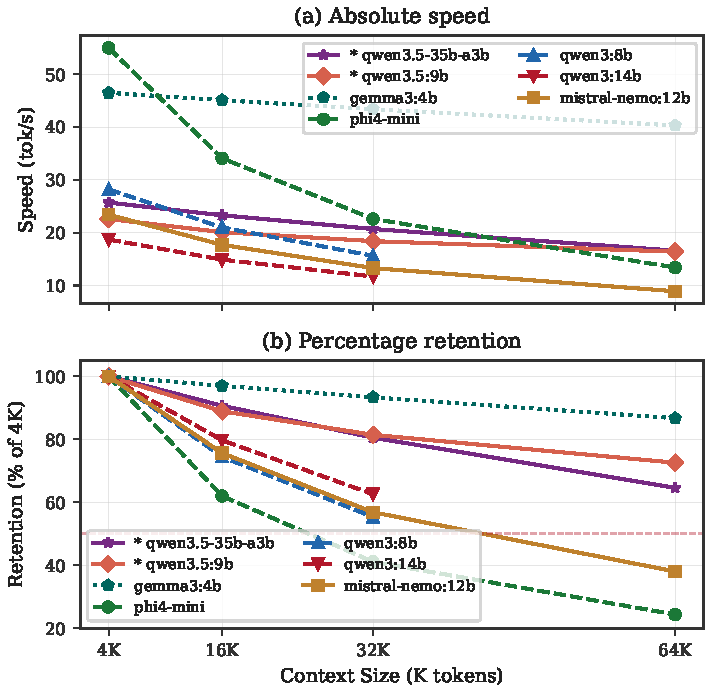
\includegraphics[width=0.86\textwidth]{figures/fig-context-degradation}
\caption{Generation speed with filled context (80\,\% real-token fill,
verified-stock 24-CU, $n{=}3$).  Panel~(a) is absolute throughput,
panel~(b) the same data as a fraction of each model's 4K throughput.
Per-cell values are in Table~7 of the main text.}
\end{figure}

\begin{figure}[h]
\centering
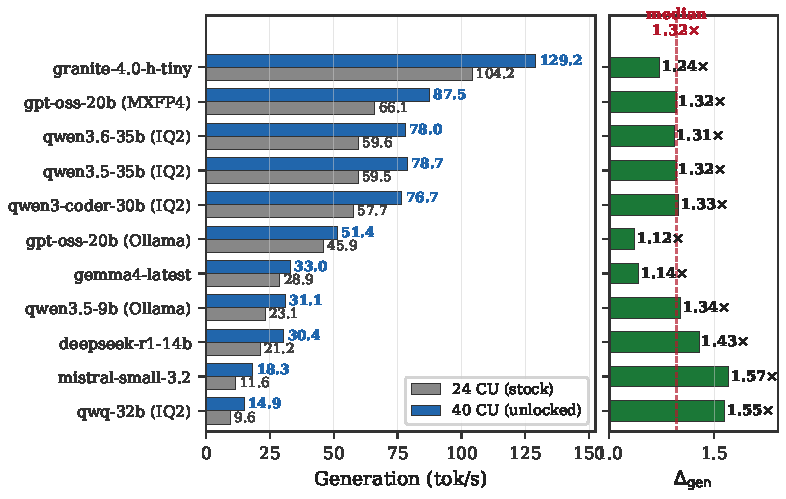
\includegraphics[width=0.86\textwidth]{figures/fig-cu-unlock}
\caption{40-CU unlock A/B on the 11-model paired subset at 4K context.
Left: generation throughput before (24~CU) and after (40~CU) the
unlock.  Right: per-model speed-up with the cohort median
(1.32$\times$) marked.  Prompt, KV width and llama.cpp build are
identical between arms.  Per-model values are in Table~14 of the main
text.}
\end{figure}

%=====================================================================
\section{Raw Data}
%=====================================================================

The following are in the project repository, not reproduced here.  They
are either bulky or only useful machine-readable: the per-second GPU telemetry CSVs sampled during the
40-CU sweeps, the concurrency contention probe, the full per-run JSON
for every table in the main text, and the 720 raw model responses from
the competence probe.  Each measurement harness is released beside its
results.

\end{document}
